\documentclass{article}
\usepackage{graphicx}
\usepackage{amsmath}
\usepackage{lipsum}
\usepackage{indentfirst}

\renewcommand{\abstractname}{Abstrak}
\renewcommand{\contentsname}{Daftar Isi}

\begin{document}

\title{Klasifikasi Tulisan Tangan Menggunakan Multi Layer Perceptron}
\author{
	Kelompok \textbf{Kosong(0)} \\
	~\\
	Laila Mauhibah - \texttt{1206208536} \\
	Pandhu Hutomo Aditya - \texttt{1206277426} \\
	Rifqi Al Fatih - \texttt{1206243476} \\
	Roland Raymond Dino - \texttt{1206249265} \\
	Thirafi Dide - \texttt{1206240814} \\
	~\\
	Fakultas Ilmu Komputer, Universitas Indonesia
}

\maketitle

\begin{abstract}
\lipsum[1]
~\\
\noindent \textbf{Kata Kunci - }Lorem, Ipsum, Dolor, Sit, Amet
\end{abstract}

\pagebreak

\tableofcontents

\pagebreak

\section{Problem Description}

	\subsection{Motivation}
	\lipsum[1]

	\subsection{Problem Definition}
	\lipsum[1]

	\subsection{Related Work}
	\lipsum[1]

\graphicspath{ {images/} }
\section{Pendekatan}
	\textit{Neural Network} merupakan suatu metode pembelajaran yang menggunakan pemodelan syaraf otak (jaringan syaraf tiruan). Motivasi sesungguhnya dalam pengembangan \textit{Artificial Neural Networks} (ANNs) adalah untuk memodelkan proses pengamatan hewan dan manusia secara kognitif. Banyak pengaplikasian ANNs yang menunjukkan bahwa pendekatan ini sangat berguna, meskipun hal ini juga membuat kita mengetahui bahwa terdapat beberapa permasalahan yang dapat dipecahkan oleh ANNs dan masalah yang tidak dapat dipecahkan oleh ANNs.
	\par Dalam \textit{paper} ini kita akan menggunakan metode \textit{Multi-layer Perceptron} untuk melakukan penelitian terhadap \textit{Digit Recognizer}. Dalam masalah \textit{Digit Recognizer} ini dideskripsikan bahwa sebuah kantor pos ingin mengirim surat secara otomatis berdasarkan kode pos. Lalu dikumpulkan sebuah data yang berisi 10000 tulisan tangan berupa angka. Setiap data memiliki label yang menandakan sebuah angka, dan 256 piksel dari angka tulisan tangan. \textit{Multi-layer Perceptron} digunakan untuk mengenali tulisan tangan yang terdapat pada kode pos tersebut.
	
	\subsection{Metodologi}
	\textit{Multi-layer Perceptron} (MLP) merupakan model yang sangat sederhana dari \textit{biological neural networks} dan didasarkan pada prinsip \textit{feed-forward-flow} yang berarti informasi yang ada hanya mengalir dari satu \textit{layer} ke \textit{layer} yang lainnya. MLP terdiri dari banyaknya \textit{layer} dalam grafik dimana setiap \textit{layer} saling berhubungan satu sama lain. Kecuali untuk \textit{layer} input, setiap \textit{layer} merupakan sebuah \textit{neuron} (atau elemen yang akan diproses) dengan fungsi aktivasi non linear. MLP menggunakan teknik pembelajaran yang disebut dengan \textit{backpropagation} untuk melatih jaringan. MLP merupakan modifikasi dari \textit{standard linear perceptron} yang dapat membedakan data dimana data tersebut tidak terpisah secara linear. \textit{Layer} yang terdapat pada input dan output disebut \textit{hidden layer}. Dari sudut pandang teoretis, kita tidak perlu mempertimbangkan lebih dari satu unuit output karena dua atau lebih unit output dapat dihasilkan dari dua atau lebih MLP secara paralel. Namun, jika terdapat output yang saling berhubungan maka dimungkinkan untuk mencapai hasil yang sama dengan nilai \textit{hidden units} yang kecil. Berikut ini merupakan ilustrasi dari proses input dan output dari MLP
	\begin{center}
		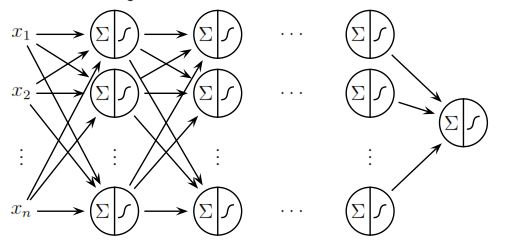
\includegraphics{images-1.jpg}
		\newline \textbf{Gambar 1. Multi-layer Perceptron}
	\end{center}
	\par Jika MLP memiliki fungsi aktivasi linear di semua \textit{neuron}, yaitu fungsi yang memetakan \textit{weighted input} untuk \textit{output} di setiap \textit{neuron}, maka dengan mudah dibuktikan dengan aljabar linear.
	Pada dasarnya perhitungan pada standar \textit{perceptron} dihitung dengan fungsi yang tidak kontinyu sebagai berikut
	\begin{center}
		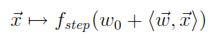
\includegraphics{equation-1.jpg}
	\end{center}
	tetapi karena beberapa alasan, \textit{neuron} pada MLP menghitungnya dengan varian yang sudah dirapikan seperti berikut
	\begin{center}
		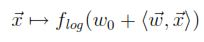
\includegraphics{equation-2.jpg}
	\end{center}
	dengan
	\begin{center}
		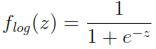
\includegraphics{equation-3.jpg}
	\end{center}
	Maka akan terdapat perbedaan antara perhitungan yang dilakukan oleh \textit{standard perceptron} dengan perhitungan yang sudah dimodifikasi dengan MLP sebagai berikut
	\begin{center}
		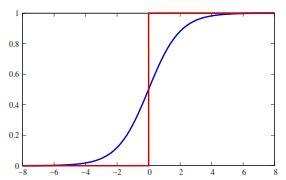
\includegraphics{graphic-1.jpg}
		\newline \textbf{Gambar 2. Perbedaan fungsi step dan sigmoid}
	\end{center}
	Flog sering disebut dengan \textit{logistic function}. \textit{Locistic function} ini merupakan fungsi yang \textit{hyperbolic tangent} dan memiliki \textit{range} diantara 0 sampai 1.
	\par Neuron dengan \textit{logistic activation} hanya dapat mengeluarkan output diantara 0 dan 1. Untuk mendapatkan output dengan jarak yang lebih besar maka kita dapat menggunakan \textit{neuron} dengan \textit{tanh activation}
	\begin{center}
		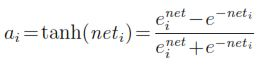
\includegraphics{equation-4.jpg}
	\end{center}
	maka didapatkan grafik perbedaan antara \textit{linear activation} dengan \textit{tanh activation}
	\begin{center}
		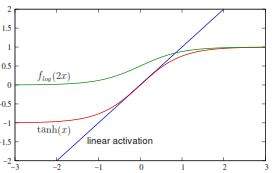
\includegraphics{graphic-2.jpg}
		\newline \textbf{Gambar 3. Perbedaan fungsi linear, logistik dan tanh}
	\end{center}
	Perhitungan jaringan output mirip dengan kasus aktivasi logistik tetapi \textit{range} yang dihasilkan lebih besar yaitu antara -1 dan 1.

	\subsection{Algoritma}
	Berikut ini merupakan algoritma yang digunakan oleh \textit{Multi-layer Perceptron}
	\begin{center}
		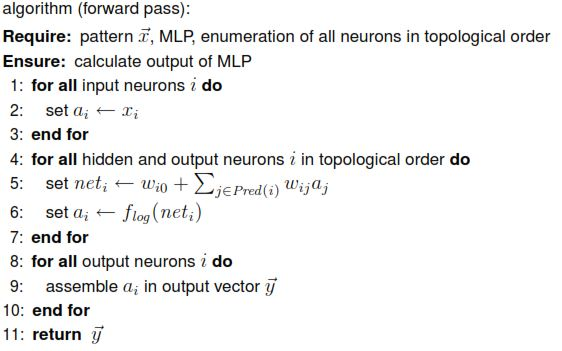
\includegraphics{images-2.jpg}
		\newline \textbf{Gambar 4. MLP Pseudocode}
	\end{center}



\section{Implementasi}
Implementasi program dibagi menjadi kelas abstraksi multilayer perceptron(MLP) dan kelas untuk membangun model MLP.\\ 
Kelas yang terdapat abstraksi MLP terdapat pada file MLP.java yang bersumber pada http://physionet.org/challenge/2010/sources/Luiz-Silva/MLP.java.\\
Kelas untuk membangun model MLP diimplementasi pada Tester.java. Pada kelas ini 
\lipsum

\section{Eksperimen}

	\subsection{Persiapan Eksperimen}
	\lipsum[1]

	\subsection{Skema Perbandingan}
	Eksperimen akan dilakukan dengan membandingkan banyaknya unit di \textit{hidden layer} dan dampaknya terhadap unit 

	\subsection{Hasil dan Analisis}
	\lipsum[1]


\section{Kelebihan dan Kekurangan}
\lipsum

\section{Kesimpulan}

	\subsection{Ringkasan}
	\lipsum[1]

	\subsection{Arahan Kedapan}
	\lipsum[1]


pros 
	dapat memecahkan pasalah yang kompleks, nonlinear
	dapat beradaptasi dengan beberapa jenis training data

cons 
sulit diimplementasi dan diinterpretasi
	tersedia software yang menyediakan built-in solusi.
sulit menentukan aritektur dari jaringan
	banyaknya layer
	banyaknya node pada layer
		tergantung kepada kompleksitas dari input dan output mapping. 
		terlalu sedikit backpropagation algorithm gagal menuju konvegen minimun saat training 
		terlalu banyak overfitting hasil training data dan performa generalisasi buruk
kompleksitas backpropagation tinggi (curse of dimentionality)
	jika dimensi data bertambah, maka jumlah data training yang diperlukan juga signifikan bertambah


	% $$http://www.researchgate.net/profile/Stephen_Dorling/publication/263416087_Artificial_neural_networks_(the_multilayer_perceptron)-a_review_of_applications_in_the_atmospheric_sciences_-_application_for_wind_retrieval_from_spaceborne_scatterometer_data/links/00b495364b91edd43a000000.pdf$



\pagebreak

\section{Appendix}

	\subsection{Data sets}
	\lipsum[1]

	\subsection{Source Codes}
	\lipsum[1]

	\subsection{Implementation Guidelines}
	\lipsum[1]


\end{document}